\documentclass[11pt]{article}

\usepackage[margin=1in]{geometry}
\usepackage[T1]{fontenc}
\usepackage{lmodern}
\usepackage{microtype}
\usepackage{booktabs}
\usepackage{graphicx}
\usepackage{amsmath}
\usepackage{amssymb}
\usepackage{caption}
\usepackage{subcaption}
\usepackage{xcolor}
\usepackage[colorlinks=true,linkcolor=linkblue,citecolor=linkblue,urlcolor=linkblue]{hyperref}
\usepackage{titlesec}
\usepackage{enumitem}

\definecolor{linkblue}{HTML}{2A78D6}
\definecolor{shade}{HTML}{F2F2F0}

\titleformat{\section}{\large\bfseries}{\thesection}{0.6em}{}
\titleformat{\subsection}{\normalsize\bfseries}{\thesubsection}{0.6em}{}
\captionsetup{font=small,labelfont=bf}
\setlist{itemsep=2pt,topsep=3pt,parsep=0pt}

\newcommand{\td}{\texttt{token\_difr}}
\newcommand{\ce}{\texttt{cross\_entropy}}
\newcommand{\ad}{\texttt{activation\_difr}}
\newcommand{\tl}{\texttt{token\_toploc}}

\title{\bfseries Checking That an Inference Provider Ran the Model It Charged You For\\[2mm]
\large What works, what it costs, and how easily the measurement lies to you}
\author{\normalsize A summary of the \texttt{inference-verification} (\texttt{ivgym}) experiments,\\
\normalsize with new measurements run for this report on a single NVIDIA H100-80GB}
\date{August 2026}

\begin{document}
\maketitle

\begin{abstract}
\noindent
You rent inference from a provider. It promises to run a specific model with
specific sampling settings, and it bills you accordingly. Nothing stops it from
quietly serving a 4-bit copy, a smaller model, or a different sampler and pocketing
the difference. This report summarizes an experimental study of whether a client can
catch that, using a testbed (\texttt{ivgym}) that pits provider-side deviations
against verifier-side detectors on real models on a GPU.

Three findings organize everything else. First, \textbf{the honest verifier works,
but only barely, and at a price}: recomputing the reference model and comparing
per-token sampling margins catches every deviation we tried on some model, but no
single detector is reliable across model families, and the per-token signal from
realistic quantization is so weak ($d' \approx 0.07$) that thousands of tokens must
be pooled before a decision is trustworthy. Second, \textbf{most of the cheap
alternatives fail in a specific and predictable place}: a client-side proxy model
catches wholesale model substitution at AUC 0.998 without ever running the
reference, but is blind to quantization, because quantization moves the served
distribution less than the reference model's own run-to-run nondeterminism. Third,
and least expected: \textbf{the dominant error in this literature-adjacent
measurement is statistical, not cryptographic}. Resampling evaluation batches from
too small a token pool inflates detection AUC arbitrarily; we show the same
measurement reading 0.98 and 0.53 depending only on pool size, and re-measure the
testbed's headline table inside a valid regime, where 16 of 24 cells fall by up to
0.46 AUC and two apparent detector capabilities turn out not to exist. The same
correction dissolves the study's reported ``detector reversals'': re-measured, none
of them has a negative per-token effect size, and the detectors that appeared to
point the wrong way are simply at chance. On a 56{,}160-token pool --- large enough
to test the prediction for the first time --- the per-token effect size forecasts the
batch at which detection arrives to within 0.03 AUC.

We also report two negative results that we believe generalize. A learned,
calibrated per-token ``value'' head and a formally-derived information-directed
matched filter both fail to beat a hand-written entropy heuristic, while a
hardware-aware prefix scheduler --- which is pure cost geometry and contains no
statistics at all --- gives a $16\times$ wall-clock saving. In selective
verification, the cost side transfers and the signal side does not.
\end{abstract}

\section{The problem}

An inference provider and a client agree on a \emph{specification} $\phi$: a model
$M$ and its sampling parameters (temperature, top-$k$, top-$p$, and a seed). The
provider returns \texttt{(prompt, output)} pairs and claims they came from running
$\phi$ on $M$. It may instead have run something cheaper. The deviations that matter
economically are not exotic:

\begin{itemize}
\item \textbf{Serve a smaller model.} Bill for a 4B, serve a 0.6B. This is the
      highest-value cheat --- here, $6.7\times$ fewer FLOPs.
\item \textbf{Quantize.} Serve the right model at 4-bit or with an fp8 KV cache.
      Subtle, and cheap to do.
\item \textbf{Change the sampler.} Wrong temperature, wrong seed, or a plain bug
      that truncates the candidate set.
\end{itemize}

The client's problem is that it only sees text. It cannot audit the provider's
hardware, and the provider is exactly the party whose self-reports cannot be
trusted --- so any verifier that needs the provider's cooperation (a reported trace,
a logged KV cache) is one the provider can stub out. Zero-knowledge proofs of
inference solve this in principle and are many orders of magnitude too slow in
practice.

The approach studied here follows DiFR \cite{difr}: the client \emph{recomputes}. It
runs $M$ itself over \texttt{prompt + claimed\_tokens}, and asks whether each
claimed token is what $\phi$ on $M$ would have produced. The complication that makes
this a research problem rather than an equality check is \textbf{nondeterminism}:
batching, kernel selection, and reduction order all change logits slightly, so
honest outputs do not reproduce bit-exactly. Verification is therefore a hypothesis
test, not a comparison.

\paragraph{What this report is.} The \texttt{ivgym} testbed makes the two sides of
that test pluggable --- attacks (provider deviations) and defenses (per-token
divergence scores) --- and holds the evaluation protocol fixed, so ``who catches
whom'' is a grid rather than an anecdote; the design follows the model-organism
testbed pattern \cite{clymer}, in which known deviations are planted so that a
detector's misses are observable. This report summarizes what that grid says
across roughly two dozen experiments on Qwen3, Llama-3.x, SmolLM2, Pythia and GPT-2
models, and adds five new measurements, run for this report, that close the largest
gaps in the existing record. New results are marked \textbf{[new]}.

\section{Setup: the game, and the number we report}
\label{sec:setup}

\paragraph{The players.} The \textbf{provider} generates under a spec of its
choosing while claiming $\phi$. The \textbf{verifier} recomputes under $\phi$ and
emits a per-token divergence score $s_t \ge 0$, higher meaning ``less consistent
with $\phi$ on $M$''. The verifier never sees the attack. Provider and verifier
share a per-position seed for the Gumbel noise used in sampling, so under the
default detector an honest token scores exactly $0$ whenever the verifier's own
argmax agrees with the claimed token --- which is the common case, about 98\% of
honest tokens --- and a positive post-Gumbel margin otherwise.

\paragraph{Four detectors.} \td{} is the post-Gumbel margin above; \ce{} is the
negative log-likelihood of the claimed token; \ad{} is an $L_2$ distance on randomly
projected activations; \tl{} is the rank of the claimed token in the verifier's
filtered distribution (no seed synchronization needed). All four require recomputing
$M$. A separate family of \emph{black-box} detectors scores
\texttt{(prompt, tokens)} without running $M$ at all, using a small proxy model or
no model.

\paragraph{From a token score to a decision.} A single token is far too noisy to
classify. The protocol is fixed once for every experiment: split honest tokens into
disjoint calibration and evaluation halves; winsorize at the 99.9th percentile of
the calibration half so one outlier cannot carry a batch; average $b$ tokens into a
batch statistic $S$; and flag when $S > \tau$, with $\tau$ set to the
$(1-\alpha)$ quantile of the calibration half's batch statistics.

\paragraph{The metric.} We report the \textbf{standardized partial AUC at
FPR $\le 0.5\%$}. A provider is not a one-shot bet --- it is checked continuously,
so it cannot tolerate more than a sliver of false accusations. Restricting the ROC
to that region and McClish-standardizing it keeps the familiar scale (0.5 = chance,
1.0 = perfect) while measuring only the operating region a verifier can actually
use. It is consistently \emph{stricter} than full-range AUC. Every number in this
report is this quantity unless stated otherwise, and unless noted every new number
is a mean $\pm$ standard deviation over 5 protocol seeds.

\section{The measurement trap, and how to stay out of it}
\label{sec:trap}

We put this first because it changes how to read every other table, including
several published in the testbed's own documentation.

\subsection{Batches resampled from a small pool inflate AUC without bound}

The batch statistic $S$ is a mean of $b$ tokens drawn \emph{without replacement from
a fixed token pool}. As $b$ approaches the pool size, every batch mean converges to
the pool mean and the honest variance collapses. The AUC then no longer answers
``would a fresh batch be flagged?'' --- it answers ``do these two particular pools
have different means?'', which is nearly deterministic. Worse, it is deterministic
in \emph{both} directions: whichever pool mean happens to be larger drives the AUC
toward 1.0 or toward 0.0.

The testbed's own diagnostic makes this vivid on one cell. Holding the model, the
attack, and the per-token scores fixed and growing only the pool, \td{} versus
\texttt{quant\_4bit} on Qwen3-1.7B reads:

\begin{center}\small
\begin{tabular}{rrl}
\toprule
honest pool (tokens) & batch / null split & AUC @ FPR $\le 0.5\%$ \\
\midrule
576    & 69.4\% & $0.977 \pm 0.010$ \\
1{,}152  & 34.7\% & $0.577 \pm 0.042$ \\
2{,}304  & 17.4\% & $0.679 \pm 0.099$ \\
4{,}608  & 8.7\%  & $0.523 \pm 0.021$ \\
9{,}216  & 4.3\%  & $0.524 \pm 0.012$ \\
22{,}464 & 1.8\%  & $0.530 \pm 0.011$ \\
\bottomrule
\end{tabular}
\end{center}

\noindent 0.977 and 0.530 are the same measurement. Note that the approach is not
smooth: at 17.4\% the reading bounces back to 0.679 with a $\pm 0.099$ spread across
protocol seeds. Over-ratio measurements are not conservatively biased, they are
erratic, which is why the failure is hard to spot from a single table. The rule of
thumb that falls out is to keep the batch well under $\approx$10\% of the honest
evaluation split, and to watch the seed-to-seed spread as the tell.

The pool-independent way to state a deviation's strength is the per-token
standardized effect size $d' = (\mathbb{E}[s \mid \text{deviating}] -
\mathbb{E}[s \mid \text{honest}]) / \mathrm{sd}(s \mid \text{honest})$; a batch of
$b$ independent tokens separates by $d'\sqrt{b}$. For \texttt{quant\_4bit} on this
model $d' = 0.0716$, which is tiny, and which predicts that AUC 0.90 needs
$b \approx 2{,}766$ --- and hence a pool of at least 55{,}000 tokens to stay inside
the ratio ceiling. That prediction was left untested, because no pool that large had
been generated.

\subsection{[new] The headline grid, re-measured inside the ceiling}
\label{sec:headline}

The testbed's front-page table --- 6 attacks $\times$ 4 detectors on Qwen3-0.6B ---
was measured at a \textbf{78\%} ratio, and had never been re-run. We generated a
117 prompt $\times$ 192 token pool (22{,}464 tokens per configuration) and scored
every cell twice from the \emph{same} per-token scores: once over the full pool at
batch 1000 (an 8.9\% ratio, legitimate), and once over a sub-pool of the first 20
sequences $\times$ 128 tokens at the same batch (a 78\% ratio --- the published
configuration, reproduced as a sub-pool so that the pool size is the only thing that
differs).

\begin{table}[h]
\centering\small
\begin{tabular}{lrrrrrrrr}
\toprule
attack & \multicolumn{2}{c}{\td} & \multicolumn{2}{c}{\ce} & \multicolumn{2}{c}{\ad} & \multicolumn{2}{c}{\tl} \\
\cmidrule(lr){2-3} \cmidrule(lr){4-5} \cmidrule(lr){6-7} \cmidrule(lr){8-9}
 & 78\% & 8.9\% & 78\% & 8.9\% & 78\% & 8.9\% & 78\% & 8.9\% \\
\midrule
\texttt{quant\_4bit} & 0.908 & 0.718 & 0.565 & 0.505 & \textbf{1.000} & \textbf{1.000} & 0.732 & 0.600 \\
\texttt{kv\_fp8} & 0.576 & 0.511 & 0.597 & 0.507 & \textbf{1.000} & \textbf{1.000} & 0.679 & 0.517 \\
\texttt{temp\_1.1} & 0.596 & 0.516 & \textbf{0.897} & \textbf{0.823} & 0.551 & 0.504 & 0.808 & 0.661 \\
\texttt{seed\_43} & \textbf{1.000} & \textbf{1.000} & 0.987 & 0.524 & 0.499 & 0.575 & 0.828 & 0.507 \\
\texttt{bug\_k2} & \textbf{0.695} & \textbf{0.553} & 0.499 & 0.510 & 0.618 & 0.499 & 0.501 & 0.523 \\
\texttt{bug\_k32} & \textbf{0.992} & \textbf{0.712} & 0.590 & 0.605 & 0.499 & 0.499 & 0.912 & 0.686 \\
\bottomrule
\end{tabular}

\caption{[new] The testbed's headline grid, scored twice from the \emph{same}
per-token scores: at the published 78\% batch/pool ratio and at a legitimate
8.9\% ratio. Qwen3-0.6B, 22{,}464-token pool, batch 1000, mean over 5 protocol
seeds (standard deviations in the text). \textbf{Bold} marks the detector a
portfolio would pick for that attack --- the same one in both arms, in every row.
Figure~\ref{fig:ratio}A plots the same 24 cells.}
\label{tab:headline}
\end{table}

Sixteen of the 24 cells fall, by a median of 0.137 and by as much as 0.463. Three
are saturated at 1.000 in both arms, and five \emph{rise} --- the artifact's other
tail. Four of the five are within 0.08 of chance in both arms, which is what a
collapsed-variance measurement pushed the wrong way looks like; the fifth is the
one cell where \ce{} has a real signal to report ($d' = 0.133$ on
\texttt{bug\_k32}), and there the small pool happened to \emph{understate} it,
0.590 against 0.605. The artifact does not have a sign.
Averaged over the grid, the seed-to-seed standard deviation is three times larger
in the inflated arm ($0.041$ versus $0.013$). The small-pool measurement is not
merely optimistic; it is unstable, because what it reports is a property of the
particular pool it drew.

The re-measurement is conservative about what it overturns. The winning detector
is unchanged in all six rows, so the portfolio recommendation of
Section~\ref{sec:deploy} survives intact. What changes is how good the winner is:
the floor across the six attacks drops from 0.695 to 0.553, and \td{} --- which at
78\% clears AUC 0.90 on three of six attacks, the basis for calling it the strong
general detector --- clears it on one.

\paragraph{The valid arm is not just the pessimistic reading; it is the correct
one.} Two cells settle this. Under \texttt{seed\_43} the provider redraws from
\emph{exactly} the honest distribution, so a detector that only reads where the
claimed token sits in that distribution has, mechanistically, nothing to see. At
78\%, \ce{} reads 0.987 and \tl{} reads 0.828 --- near-perfect detection of a
deviation neither can in principle observe. At 8.9\% they read 0.524 and 0.507,
which is the answer the mechanism requires. On these cells the inflated arm did not
exaggerate a real signal, it manufactured one. That is a sharper argument than
``smaller numbers are safer'': the ratio ceiling is a correctness condition, and
the grid contains its own falsification test for it.

One cell moves the other way and we cannot fully account for it. \ad{} on
\texttt{seed\_43} goes from 0.499 to $0.575 \pm 0.021$, with a per-token
$d' = +0.057$. \ad{} compares projected activations recomputed on the same claimed
prefix, so the seed should be invisible to it. We attribute the residual to the
honest and re-seeded pools containing different \emph{text}, so the two
nondeterminism floors are not sampled over identical contexts --- a pool-composition
effect rather than sampler sensitivity --- but the ablation that would settle it was
not run. The only genuine per-token reversals anywhere in the grid are \ad{} on
\texttt{bug\_k2} ($d' = -0.008$) and on \texttt{bug\_k32} ($d' = -0.032$), and both
are small enough to read as chance in both arms.

\subsection{[new] Does the effect size predict when detection arrives?}
\label{sec:poolscaling}

Section~\ref{sec:trap} left a prediction untested for want of a pool: at
$d' \approx 0.07$, \td{} versus \texttt{quant\_4bit} should reach AUC 0.90 at a
batch of roughly 2{,}800, which needs at least 55{,}000 honest tokens to stay under
the ratio ceiling. We generated one --- 117 prompts $\times$ 480 tokens on
Qwen3-1.7B, \textbf{56{,}160 evaluation tokens}, a 28{,}080-token honest null split,
5 protocol seeds --- and swept the batch across it. The measured per-token effect
size is $d' = 0.0776$, which puts the AUC-0.90 batch at 2{,}361, inside the ceiling
for this pool for the first time.

\begin{table}[h]
\centering\small
\begin{tabular}{rrlrl}
\toprule
batch $b$ & ratio & measured AUC & predicted & residual \\
\midrule
200 & 0.7\% & $0.531 \pm 0.007$ & 0.520 & $+0.011$ \\
400 & 1.4\% & $0.559 \pm 0.010$ & 0.548 & $+0.011$ \\
800 & 2.8\% & $0.627 \pm 0.015$ & 0.625 & $+0.002$ \\
1{,}600 & 5.7\% & $0.781 \pm 0.023$ & 0.790 & $-0.010$ \\
2{,}361$^{\dagger}$ & 8.4\% & $0.873 \pm 0.008$ & 0.900 & $-0.027$ \\
5{,}600 & 19.9\% & $0.996 \pm 0.002$ & 0.998 & $-0.003$ \textit{over ceiling} \\
11{,}200 & 39.9\% & $1.000 \pm 0.000$ & 1.000 & $+0.000$ \textit{over ceiling} \\
\bottomrule
\end{tabular}

\caption{[new] Detection arriving on schedule. Qwen3-1.7B, \td{} versus
\texttt{quant\_4bit}, one 56{,}160-token pool, batch swept, 5 protocol seeds.
``Predicted'' is $\Phi(d'\sqrt{b}/\sqrt{2})$ mapped through the same partial-AUC
definition, using only the pool-independent per-token effect size.
$^{\dagger}$ the batch the effect size nominates for AUC 0.90. The last two rows
exceed the 10\% ratio ceiling and are shown for completeness.
Plotted in Figure~\ref{fig:ratio}B.}
\label{tab:poolscaling}
\end{table}

The prediction holds. Across the five points inside the ceiling the mean absolute
residual is 0.012 and the worst is 0.027, and at the nominated batch the
measurement reads $0.873 \pm 0.008$ against a predicted 0.900. The residual is
signed the way theory says it should be: the prediction treats the $b$ tokens in a
batch as independent, and tokens inside a sequence are not, so it should be mildly
optimistic exactly where the curve is steep. Read as a design tool, the effect size
gives a good estimate of the batch a verifier needs and a slight under-estimate of
it. The two over-ceiling rows are consistent but uninformative --- by then the true
AUC is saturated, so the artifact has nothing left to inflate.

The deployment consequence is the blunt part. A 4-bit quantization of a 1.7B model
is detectable --- but the verifier needs on the order of $10^3$ tokens pooled into
each verdict and $10^4$--$10^5$ honest tokens to calibrate the threshold against.
That is not a few hundred tokens of one response; it is a continuous relationship
with a provider, aggregated over many of them. Any protocol that promises a verdict
on a single completion is not, on this evidence, measuring quantization.

\begin{figure}[t]
\centering
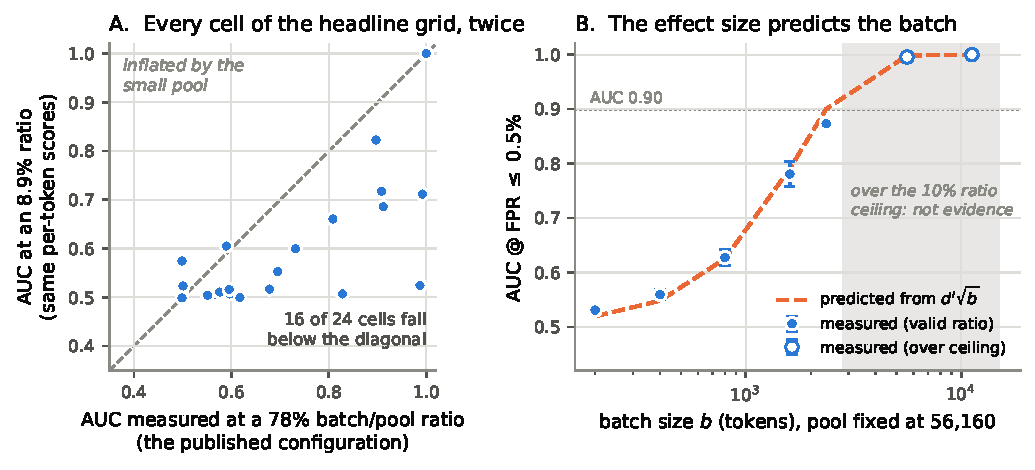
\includegraphics[width=\textwidth]{figs/fig_ratio.pdf}
\caption{[new] The measurement trap, and the measurement that escapes it.
\textbf{A:} every cell of Table~\ref{tab:headline}, plotted at the published 78\%
ratio against the same per-token scores read at 8.9\%. Points below the diagonal
were inflated by the small pool. The handful above it are the same artifact acting
in the other direction; all of them are within 0.08 of chance.
\textbf{B:} Table~\ref{tab:poolscaling} --- with the pool held fixed at 56{,}160
tokens, the batch at which detection arrives is predicted by the per-token effect
size alone, until the batch crosses the ratio ceiling and the measurement stops
being evidence.}
\label{fig:ratio}
\end{figure}

\subsection{[new] The ``detector reversal'' cells}
\label{sec:reversal}

The cross-family claim in Section~\ref{sec:catch} --- no single recompute detector
is uniformly robust --- rests on its most dramatic cells: \td{} reading 0.040 on
SmolLM2-1.7B under \texttt{kv\_fp8} and 0.086 on Pythia-410m, cells where the
divergence signal appears to \emph{reverse}, the honest side scoring higher than the
attacked side. Those cells come from a sweep run at a 52\% ratio. A collapsed-variance
measurement is pushed toward \emph{both} extremes, so ``some cells read 1.0 and some
read 0.04'' is precisely the artifact's signature, and the evidence for the robustness
claim has the same defect as the evidence it was raised against.

Reversal is a mechanistic claim, and it has a pool-independent test: the sign of the
per-token effect size. A real reversal has $d' < 0$ no matter how the batches are
drawn. We re-generated five cells --- the two reversals, a third low cell, a
mid-range cell, and a control the sweep read at 1.000 so the check is two-sided ---
at 64 prompts $\times$ 128 tokens, and scored each three ways from a single
generation pass.

\begin{table}[h]
\centering\small
\begin{tabular}{llrllr l}
\toprule
model & attack & published & re-run at 52\% &
re-run at 9.8\% & $d'$ & reversed? \\
\midrule
\texttt{SmolLM2-1.7B} & \texttt{kv\_fp8} & 0.040 & $0.601 \pm 0.093$ & $0.513 \pm 0.008$ & $+0.0188$ & no \\
\texttt{pythia-410m} & \texttt{kv\_fp8} & 0.086 & $0.499 \pm 0.000$ & $0.500 \pm 0.001$ & $+0.0011$ & no \\
\texttt{pythia-410m} & \texttt{quant\_4bit} & 0.146 & $0.501 \pm 0.002$ & $0.501 \pm 0.001$ & $+0.0101$ & no \\
\texttt{Qwen3-0.6B} & \texttt{bug\_k2} & 0.123 & $0.566 \pm 0.073$ & $0.515 \pm 0.011$ & $+0.0344$ & no \\
\texttt{Qwen3-0.6B} & \texttt{seed\_43} & 1.000 & $1.000 \pm 0.000$ & $1.000 \pm 0.000$ & $+0.6031$ & no \\
\bottomrule
\end{tabular}

\caption{[new] None of the reversals is real. Each cell re-generated at
8{,}192 tokens and scored three ways from one pass: at the sweep's own 52\%
configuration (reproduced as a sub-pool so only the pool size differs), at a
legitimate 9.8\% ratio, and by the pool-independent per-token effect size $d'$.
\td{}, 5 protocol seeds.}
\label{tab:reversal}
\end{table}

\textbf{Every cell has $d' > 0$}, including both cells the sweep reported as
reversals: the attacked side scores higher than honest on all five, which is the
direction the detector is designed to produce. Re-running the sweep's own 52\%
configuration on a fresh pool reproduces neither published number ---
SmolLM2/\texttt{kv\_fp8} comes back at $0.601 \pm 0.093$ where the sweep printed
0.040 --- and that $\pm 0.093$ is itself the diagnosis. At 52\% the seed-to-seed
spread is an order of magnitude wider than at 9.8\% ($\pm 0.008$), so 0.040 and
0.601 are two draws from the same badly-conditioned estimator rather than a
disagreement about the world. The control behaves as a control must: \texttt{seed\_43}
reads 1.000 at both ratios, with $d' = +0.60$, because a large effect is a large
effect at any pool size.

What survives is duller than the claim it replaces, and we think it is the more
useful statement. \td{} does not invert on these models. It is simply \emph{at
chance} on them --- 0.513, 0.500 and 0.515 at a valid ratio --- because an fp8 KV
cache at 8{,}192 tokens is below its detection floor, on every model we tried. That
is the recompute-dominant-boundary result of Section~\ref{sec:cheap} arriving from a
second direction, not a robustness result. The portfolio argument keeps its
mechanistic basis (each detector has a class of deviation it structurally cannot
see, and the classes differ) and loses its most quotable evidence.

\section{What recomputation catches}
\label{sec:catch}

Read at a valid ratio, the detectors have a structure that is \emph{mechanistic}
rather than statistical --- it follows from what each one is allowed to look at, and
it is the part of the picture that no amount of re-measurement changes.

\begin{itemize}
\item \textbf{\ad{} is blind to the sampler, by construction.} It compares projected
activations, which are computed before a token is drawn. Change the temperature, the
seed, or the sampler itself and the activations are unchanged, so it sits at chance.
Change the weights or the KV cache and it is the strongest detector available. This
bifurcation is exact and reproducible, and it means \ad{} alone cannot verify a
sampling specification.
\item \textbf{\ce{} needs the bulk of the distribution to move.} The likelihood of
the claimed token is a coarse summary. A deviation that flips the top-2 tokens on 1\%
of positions (\texttt{bug\_k2}) barely touches it, so it reads chance --- while a
temperature change, which moves every probability, is easy for it.
\item \textbf{\td{} is the only general one}, because it sees both the forward pass
and the draw: with a shared Gumbel seed, an honest token gives exactly zero and any
deviation gives a positive margin. General is not the same as strong --- the margin
under \texttt{kv\_fp8} is reliably positive and reliably tiny ($d' = 0.015$), which
is why Sections~\ref{sec:headline} and \ref{sec:reversal} find it at chance there.
\item \textbf{\tl{} is the practical surprise.} The rank of the claimed token in the
verifier's filtered distribution needs \emph{no seed synchronization} --- a
significantly weaker deployment requirement --- and tracks \td{} closely on most
attacks. It shares \ce{}'s blindness to \texttt{bug\_k2}.
\end{itemize}

\paragraph{No single detector is robust across model families.} A sweep over 9 models
in 4 families (Qwen3, Llama-3.2, SmolLM2, Pythia; 0.36B--4B; three different
tokenizers) $\times$ 7 attacks gives 63 cells per detector. \td{} averages 0.803, with
cells at every level down to 0.040; the other three have floors at 0.000 (\ce{}),
0.000 (\ad{}) and 0.013 (\tl{}). Taking the strongest detector per attack instead of
betting on one score lifts the minimum detectability across all 63 cells to 0.78.
That is the argument for treating detectors as a portfolio rather than picking a
winner --- and it is an argument the single-model tables cannot make, which is why a
cross-family matrix is worth its GPU-hours. Averaged over models, the hardest attacks
are \texttt{bug\_k2} (0.580) and \texttt{kv\_fp8} (0.639); a wrong seed is trivially
caught (1.000 on every model), because it changes the realized draw everywhere while
leaving the distribution alone.

That sweep ran 16 prompts $\times$ 96 tokens at batch 400, a \textbf{52\%} ratio, so
every absolute number in it --- the 0.803 average, the 0.040 floor and the 0.78
portfolio minimum alike --- sits well above the ceiling of Section~\ref{sec:trap} and
should be read as an ordering rather than a level. Section~\ref{sec:reversal}
re-measures the cells that carried the strongest version of the claim, and they do not
survive: what looked like a detector pointing the wrong way is a detector at chance,
measured badly. The portfolio recommendation stands on the mechanism above --- each
detector is structurally blind to a different class of deviation --- and not on the
existence of reversals, which on present evidence there are none of.

\section{Cheaper tiers, and exactly where each one stops}
\label{sec:cheap}

Recomputing $M$ for every claimed token costs about as much as generating them. Three
cheaper tiers were studied. They fail in the same place, for the same reason, and that
common boundary is the most useful thing in this section.

\subsection{Tier 0: no model at all, or a small proxy}

Black-box detectors score \texttt{(prompt, tokens)} without running $M$: surface
statistics, a small proxy model's surprisal, or a zero-shot LLM judge reading the
continuation. Their real value is as a \emph{control}. If outputs alone can tell an
attack from honest, the expensive recomputation is not buying information --- it is
duplicating a cheap signal. The clean case is a wrong seed: \td{} scores 1.000 while a
zero-shot Claude judge sits at its own honest-null floor (0.511 against a floor of
0.989, i.e.\ no signal at all). Re-seeding redraws from the \emph{same} distribution,
so the continuation reads as a perfectly ordinary sample to any reader of the text,
while a re-run flips which Gumbel candidate won. That gap is a quantitative proof that
the deviation is invisible in the outputs and recomputation is doing real work. The
converse is worth stating too: a \emph{high} black-box AUC is not a verifier win, it
is a statement that the attack was crude.

\subsection{The one cheap signal with a trust story: the acceptance rate}

The interesting Tier-0 detector borrows the mechanism of speculative decoding
\cite{spec}. The client holds its own small proxy $q$ (sharing $M$'s tokenizer) and
computes the rate at which $q$'s drafts would have been accepted against the served
distribution $p$. That rate is exactly an overlap:
\[
\mathrm{accept} = \mathbb{E}_{x\sim q}\!\left[\min\!\left(1, \tfrac{p(x)}{q(x)}\right)\right]
= \sum_x \min(p(x), q(x)) = 1 - \mathrm{TV}(p, q).
\]
The client \emph{owns} $q$, so $q$ is a trusted anchor even though $p$ is not. If the
provider corrupts the target ($p^* \to \hat{p}$), the rate moves from
$1-\mathrm{TV}(p^*,q)$ to $1-\mathrm{TV}(\hat{p},q)$, and the client sees the shift
against a one-time offline honest reference --- without ever running $M$. Everything
this tier can and cannot do follows from one budget: the expected proxy surprisal on
honest text is $H(M,q) = H(M) + \mathrm{KL}(M \| q)$, so $\mathrm{KL}(M\|q)$ is the
\emph{entire} signal available to any proxy detector.

\begin{itemize}
\item \textbf{It wins outright on substitution.} A provider paid for Qwen3-4B that
secretly serves Qwen3-0.6B is caught at \textbf{AUC 0.998} (honest acceptance 0.776
versus 0.700), using a trusted 1.7B draft and never running $M$ --- at $2.3\times$
fewer FLOPs than recomputation. Swapping the model moves $\mathrm{TV}(p,q)$
wholesale.
\item \textbf{It survives the standard evasion.} A provider that quantizes and then
retunes temperature to restore the honest \emph{entropy} blinds an entropy or
cross-entropy fingerprint (AUC $1.00 \to 0.59$) but cannot re-enter the honest
acceptance band, because matching entropy does not restore $\mathrm{TV}(\hat{p},q)$.
The draft-anchored axis still separates it (0.998).
\item \textbf{It is blind to realistic quantization.} At \texttt{quant\_4bit}
strength the measured acceptance-rate AUC sits near chance on real models, while
\td{} separates every attack. Quantization moves $\mathrm{TV}(p,q)$ less than the
reference model's own honest run-to-run nondeterminism.
\end{itemize}

\noindent This is the \textbf{recompute-dominant boundary}, and every cheap tier in
the study hits the same wall: \emph{deviations that change what the model can do are
cheap to catch; deviations that change only how precisely it does it are not.} A
cheap proxy shrinks how often the exact recomputation must fire. It does not replace
it.

\subsection{A richer proxy panel, and the dose-response curve}

A separate line of experiments makes the capability-detection idea quantitative on a
larger claimed model. A provider claims Qwen2.5-7B-Instruct; a verifier holding only
sub-2B proxies scores the completion with eight aggregate features (surprisal
mean/sd/max, mean log-rank, fractions of surprising ranks, mean entropy) from a single
teacher-forced pass, and a logistic detector is cross-validated over 300 Alpaca
prompts. Detectability tracks how much compute the attacker saved:

\begin{center}\small
\begin{tabular}{lrrl}
\toprule
served instead of the 7B & compute gap & panel AUC @ 128 tok & verdict \\
\midrule
Qwen2.5-0.5B & $15.4\times$ & 0.997 & caught \\
Qwen2.5-1.5B & $4.9\times$  & 0.991 & caught \\
Qwen2.5-3B   & $2.5\times$  & 0.580 & near chance \\
Qwen2.5-7B in nf4 & $1.0\times$ & 0.462 & chance \\
\bottomrule
\end{tabular}
\end{center}

\noindent The cliff sits between a $5\times$ and a $2.5\times$ downgrade, at a
verification cost of about 27\% of \emph{one} claimed-model forward pass. This detector
also proved hard to evade by sampling tricks: an attacker tuning temperature to match
honest cross-entropy collapses a mean-cross-entropy detector to 0.65 while the panel
holds at 0.99; searching a temperature $\times$ top-$p$ grid for the panel's weakest
point never pushes it below 0.995; paraphrasing the cheap model's output with itself
moves it from 0.997 to 0.990. Two benign perturbations of the honest provider's
numerical stack (kernel and batch changes; then fp32 instead of bf16) shift the
features measurably --- an honest-versus-honest classifier reaches 0.76 --- but along a
direction the capability detector ignores, so false positives stay at nominal
(3.3\% and 5.0\% against a 5\% budget) and detection is unaffected.

Substituting a model along an ordered ``distance'' ladder gives the same shape: a
quantized copy of $M$ is at chance to a cheap proxy, and AUC climbs monotonically with
distance, crossing the useful range (${\approx}0.85$) only once the substitute has a
different post-training lineage or a different family --- and this holds even when the
proxy's tokenizer differs from $M$'s.

\paragraph{A note on comparability.} These panel numbers are full-range
cross-validated ROC-AUC on greedy decoding over a fixed prompt set --- a different and
more forgiving protocol than the FPR-constrained partial AUC used everywhere else in
this report. They should be read as a separate line of evidence about capability
detection, not as entries in the same table.

\section{What a selective audit really costs}
\label{sec:cost}

If a full audit is too expensive, audit some tokens. The natural implementation ranks
tokens by a cheap proxy signal and recomputes the top fraction. The fraction of tokens
audited then gets reported as the cost. \textbf{It is not the cost}, and the gap is
large enough to invert conclusions.

Reading $M$'s logits at generated position $j$ requires a prefill over
\texttt{prompt + claimed[:j]}. So a sequence's audit cost is set by its \emph{deepest}
audited position, and any sequence touched at all re-pays for its prompt. A global
top-$k$ rule scatters its audit across essentially every sequence, which means it pays
nearly every prefill in order to score a few tokens. Measured on a backend instrumented
to prefill lazily and refuse to serve an unpaid row (64 sequences $\times$ 128 tokens,
Qwen3-1.7B):

\begin{center}\small
\begin{tabular}{lrrrr}
\toprule
& \multicolumn{2}{c}{global top-$k$} & \multicolumn{2}{c}{prefix schedule} \\
\cmidrule(lr){2-3}\cmidrule(lr){4-5}
nominal budget & realized cost & seconds & realized cost & seconds \\
\midrule
5\%   & 75.8\% & 1.75 & 5.0\%  & 0.11 \\
10\%  & 86.4\% & 1.53 & 10.0\% & 0.21 \\
20\%  & 92.4\% & 1.51 & 20.0\% & 0.42 \\
50\%  & 97.1\% & 1.48 & 50.0\% & 0.97 \\
100\% & 100\%  & 1.48 & 100\%  & 1.49 \\
\bottomrule
\end{tabular}
\end{center}

\noindent The sharpest number here needs no statistics: \textbf{a ``5\%'' top-$k$ audit
takes 1.75 seconds, and auditing every single token takes 1.48}. The reported saving
was overstated by up to $15\times$. The fix is a scheduler that admits contiguous
per-sequence prefixes greedily by value per unit of \emph{marginal} cost --- depth is
cheap, breadth is expensive --- which spends exactly what it is budgeted and runs
$16\times$ faster at a 5\% budget. Plotted against realized cost rather than nominal
budget, one prefix-scheduled operating point (75\% of a full audit, AUC
$0.788 \pm .043$) costs strictly less \emph{and} detects 0.12--0.20 AUC more than
four separate top-$k$ points, every one of which the naive accounting would have
called cheaper. Those four separate by 1.5--4.4 combined standard deviations and
only two clear 2\,sd, so the individual comparisons are directional; the cost
difference underneath them is not.

\begin{figure}[t]
\centering
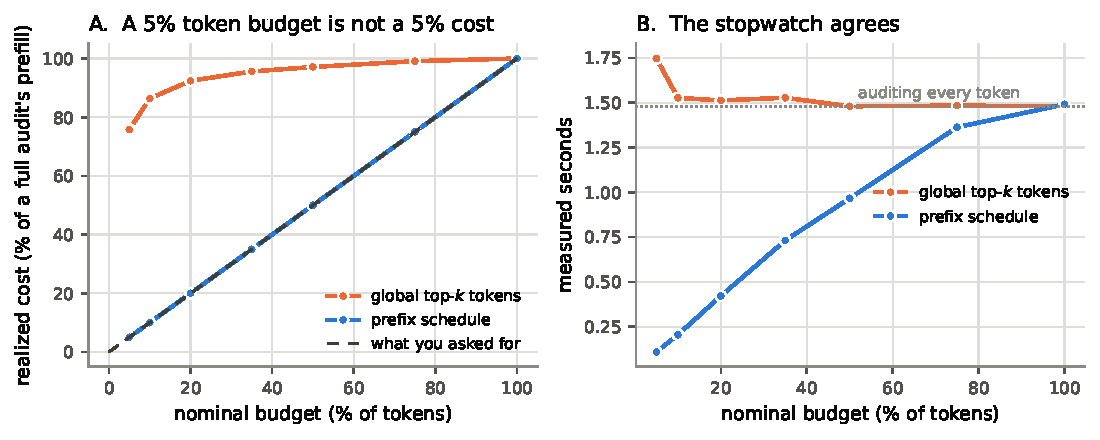
\includegraphics[width=\textwidth]{figs/fig_cost.pdf}
\caption{The audit-cost result, and the one clean positive in the study. \textbf{A:}
a global top-$k$ audit's realized prefill cost against its nominal token budget; the
prefix schedule lies on the diagonal (it is hidden under the dashed reference line,
which is the point). \textbf{B:} wall clock. Top-$k$ at a 5\% budget is slower than
auditing every token. Qwen3-1.7B, 64 sequences $\times$ 128 tokens.}
\label{fig:cost}
\end{figure}

\subsection{[new] Is the cost result about the attack, or about the geometry?}
\label{sec:prefix2}

Everything above was measured against a single deviation (\texttt{quant\_2bit}).
Two of its claims could in principle be attack-dependent, and they are worth
separating. The \emph{accounting} claim --- that a nominal token budget badly
misstates realized prefill --- should not depend on the attack at all, because
prefill cost is a function of prompt lengths, sequence count and audit depth, and
none of those know what is being detected. The \emph{Pareto} claim --- that a
prefix-scheduled point can cost less and detect more --- could easily depend on it,
because it depends on where the evidence sits in a sequence. We re-ran the whole
experiment on two further attacks, one forward-pass (\texttt{kv\_fp8}) and one
sampler-side (\texttt{bug\_k32}), holding the model, the prompts, the value signal
and the protocol fixed.

\begin{table}[h]
\centering\small
\begin{tabular}{lrrrrrrl}
\toprule
& \multicolumn{2}{c}{global top-$k$ @ 5\%} & \multicolumn{2}{c}{prefix @ 5\%}
& & \multicolumn{2}{c}{full audit} \\
\cmidrule(lr){2-3}\cmidrule(lr){4-5}\cmidrule(lr){7-8}
attack & cost & sec & cost & sec & speed-up & sec & AUC \\
\midrule
\texttt{quant\_2bit} & 75.8\% & 1.75 & 5.0\% & 0.11 & 16.0$\times$ & 1.48 & $0.823 \pm 0.050$ \\
\texttt{kv\_fp8} & 76.9\% & 1.51 & 5.0\% & 0.10 & 14.5$\times$ & 1.56 & $0.507 \pm 0.005$ \\
\texttt{bug\_k32} & 78.1\% & 1.31 & 5.0\% & 0.09 & 14.4$\times$ & 1.14 & $0.601 \pm 0.042$ \\
\bottomrule
\end{tabular}

\caption{[new] The accounting gap is a property of the schedule, not of the
deviation. Qwen3-1.7B, 64 sequences $\times$ 128 tokens, 5 protocol seeds; ``cost''
is realized prefill as a fraction of a full audit's. All three attacks are scored
on identical prompts with an identical scheduler.}
\label{tab:prefix2}
\end{table}

\textbf{The accounting result replicates exactly, and that is the expected
outcome.} At a nominal 5\% budget the global top-$k$ audit realizes 75--77\% of a
full audit's prefill on every attack, and the prefix schedule realizes 5.0\% on
every attack, for a wall-clock speed-up of $14$--$16\times$. The spread across
attacks (75.8\% versus 76.9\%) is smaller than the spread across protocol seeds
within any one of them. This is the sense in which the result ``contains no
statistics'': re-running it against a different deviation is a null experiment by
construction, and it comes back null.

\textbf{The detection result is only testable where there is detection to
allocate}, and this is where the second attack is informative in a way we did not
plan. Under \texttt{kv\_fp8} every point on both curves --- 14 operating points
across two schedulers --- lies within 0.04 of chance, including the full audit
($0.507 \pm 0.005$). There is no signal at any budget, so there is nothing for an
allocation rule to allocate well or badly, and the Pareto comparison is
undefined rather than negative. That is the same wall Sections~\ref{sec:reversal}
and \ref{sec:cheap} hit from two other directions: at $10^4$ tokens an fp8 KV cache
is simply below the recompute detection floor. We note it because a reader who saw
only the \texttt{kv\_fp8} panel might conclude the scheduler had stopped working,
when what stopped was the detector.

\begin{table}[h]
\centering\small
\begin{tabular}{lrllrll}
\toprule
attack & cost & prefix AUC & full audit & top-$k$ dom. & AUC gap & sep.\ (sd) \\
\midrule
\texttt{quant\_2bit} & 35\% & $0.811 \pm 0.069$ & $0.823 \pm 0.050$ & 5 of 7 & 0.07--0.23 & 0.8--3.2 (1) \\
\texttt{bug\_k32} & 35\% & $0.610 \pm 0.047$ & $0.601 \pm 0.042$ & 7 of 7 & 0.01--0.10 & 0.1--2.0 (2) \\
\bottomrule
\end{tabular}

\caption{[new] The honest Pareto plane, restricted to the attacks that are
detectable at all at this scale (\texttt{kv\_fp8} is excluded: its full audit reads
$0.507 \pm 0.005$, so every comparison over it is noise against noise). ``Dominated''
counts global top-$k$ operating points that cost strictly more \emph{and} detect
strictly less than the single prefix-scheduled point in column 2.}
\label{tab:prefix2pareto}
\end{table}

\textbf{Where there is signal, the ordering replicates --- directionally.}
\texttt{bug\_k32} is barely detectable at this scale (a \emph{full} audit reads
$0.601 \pm 0.042$), which makes it a demanding test rather than an easy one. Its
best prefix point spends 35\% of a full audit's prefill and reads
$0.610 \pm 0.047$ --- matching or beating \emph{every} global top-$k$ point, all
seven of which cost between 78\% and 100\%. The shape is the same as
\texttt{quant\_2bit}'s: the scheduler reaches the full-audit AUC at roughly a third
of the price, and the top-$k$ curve does not reach it at any price below 100\%.

We are deliberate about how strong a claim that is. The cost half is not in doubt:
a 2--3$\times$ difference in realized prefill and a 14--16$\times$ difference in
wall clock are far outside any seed-to-seed variation. The detection half is
directional. Taking the two arms as unpaired and combining their standard
deviations, the individual dominances separate by 0.1--3.2 sd, and only three of
the twelve clear 2\,sd (Table~\ref{tab:prefix2pareto}, last column). What
replicates is the \emph{pattern} --- on both detectable attacks, a prefix point at
about a third of the cost sits at or above the entire top-$k$ curve --- not any
single pairwise comparison. Five to nine protocol seeds on an $8{,}192$-token pool
is not enough to resolve one, which is the limitation of
Section~\ref{sec:limits} showing up exactly where we would expect it.

A cheap sanity check on the exclusion in Table~\ref{tab:prefix2pareto}: run the
same dominance count on \texttt{kv\_fp8} anyway and the prefix point ``dominates''
7 of 7 top-$k$ points too --- with gaps of 0.002--0.028 and separations below
1.6\,sd. Counting dominated points is meaningless when both curves are flat on
chance, which is precisely why the attack is excluded rather than reported as a
third success.

\begin{figure}[t]
\centering
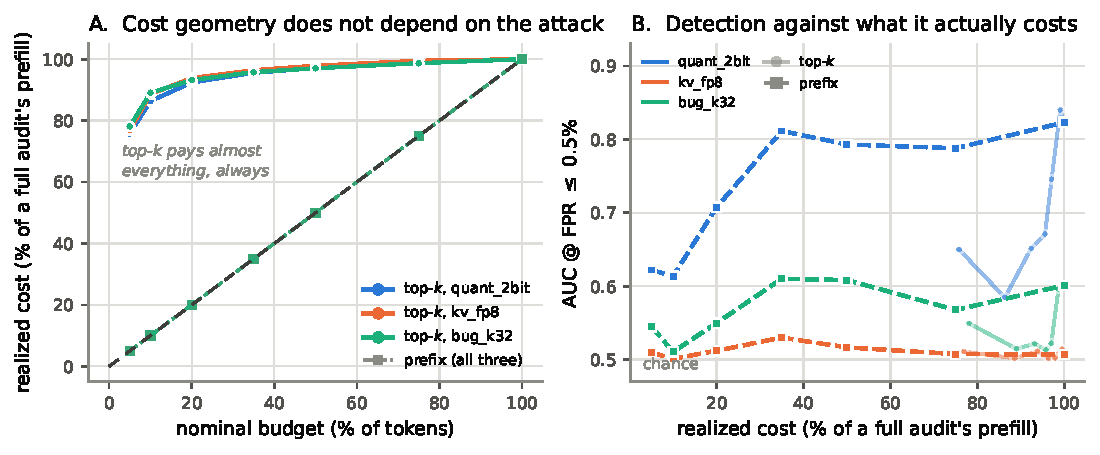
\includegraphics[width=\textwidth]{figs/fig_prefix_attacks.pdf}
\caption{[new] \textbf{A:} the accounting gap for every attack, with the prefix
schedules (dashed) on top of one another along the diagonal. The curves are
indistinguishable because prefill cost does not depend on what is being detected.
\textbf{B:} the same runs in the only plane that is honest about price --- detection
against realized cost, not against nominal budget. Under \texttt{kv\_fp8} both
schedulers sit flat on the chance line at every price.}
\label{fig:prefix2}
\end{figure}

\section{Two things that did not transfer}
\label{sec:negative}

Given a budget to spend, where should it go? Two principled answers were implemented
and both lost to a one-line heuristic. We report them because the pattern they form is
more useful than either result alone.

\subsection{A learned, calibrated per-token value head}

The first ports the confidence head from DSpark \cite{dspark}: a logistic model over
nine cheap proxy-side features (entropy, R\'enyi-2, tie margin, log top-1, top-5 mass,
surprisal, log rank, log support, relative position), trained with cross-entropy
against per-token \emph{sensitivity} --- how much the detector's score moves under a
generic zero-mean logit probe --- using \textbf{honest data only}, then temperature
scaled. It is a strict generalization of the hand-written signals: two of its features
reproduce the existing \texttt{entropy} and \texttt{tie\_margin} rules exactly.

It does not win. Against \texttt{entropy}, the library's existing default, it leads
one budget row out of six by well under two standard deviations, and \texttt{entropy}
leads two. Used instead as the value term inside the prefix scheduler --- the role
DSpark actually uses it for --- it leads one row of seven, \texttt{entropy} three,
with no pair separating by 2\,sd anywhere. Its calibration stage buys nothing: the
fitted temperature is 0.975, and on a held-out honest split the expected calibration
error gets \emph{worse} ($0.0190 \to 0.0246$). A head trained with cross-entropy
against the same label the reliability curve scores is already calibrated.

The informative part is what it learned. It puts its largest positive weights on
tie-ness ($+0.86$) and proxy surprisal ($+0.80$), and a \textbf{negative} weight on
entropy ($-0.28$) --- while \texttt{entropy} is the best allocator in the table. The
head is not failing to fit; it is fitting the wrong target. Per-token sensitivity is
not the quantity that maximizes batch-level detection.

\subsection{[new] The correct target, derived --- and it still loses}

That diagnosis has a clean fix on paper. For a weighted, centered batch statistic, the
detection power of an audited set $A$ is
\[
\delta^2(A) = \frac{b}{n}\sum_{t \in A} I(t), \qquad
I(t) = \frac{\Delta(t)^2}{v(t)},
\]
with $\Delta(t)$ the mean shift the deviation causes at position $t$ and $v(t)$ that
position's \emph{honest} variance --- the local nondeterminism. Sensitivity is the
numerator only. A near-tie position is sensitive \emph{and} noisy, so ranking on
$\Delta$ buys both, which is exactly the failure above. The theory also names the
optimal aggregator: the matched filter $w = \Delta/v$, in place of the plain mean every
number in this study is computed with.

We ran this at full scale for this report (Qwen3-1.7B, 64 prompts $\times$ 128 tokens,
batch 400 at a 9.8\% ratio, 9 protocol seeds), crossing 7 allocation rules with 3
aggregation rules, including oracle arms that read $\Delta$ and $v$ off labelled
honest/attack pairs so that a negative result would be diagnosable.

\textbf{It loses, and so does the oracle.} Holding the allocation at the derived $I$
ranking, the matched filter is \emph{below} the plain mean at every budget (at a 5\%
budget, $-0.078 \pm .008$, $t = -10.4$ paired by seed), and substituting oracle weights
does not rescue it ($-0.142 \pm .024$, $t = -6.0$ against the plain mean). Two of the
comparisons deserve to be stated plainly: even with labels for free, the derived
aggregator is worse than averaging, and the theory arm that predicts the whole
detection-versus-budget curve from the information captured overshoots the oracle
measurement by 0.24 AUC on average.

\begin{figure}[t]
\centering
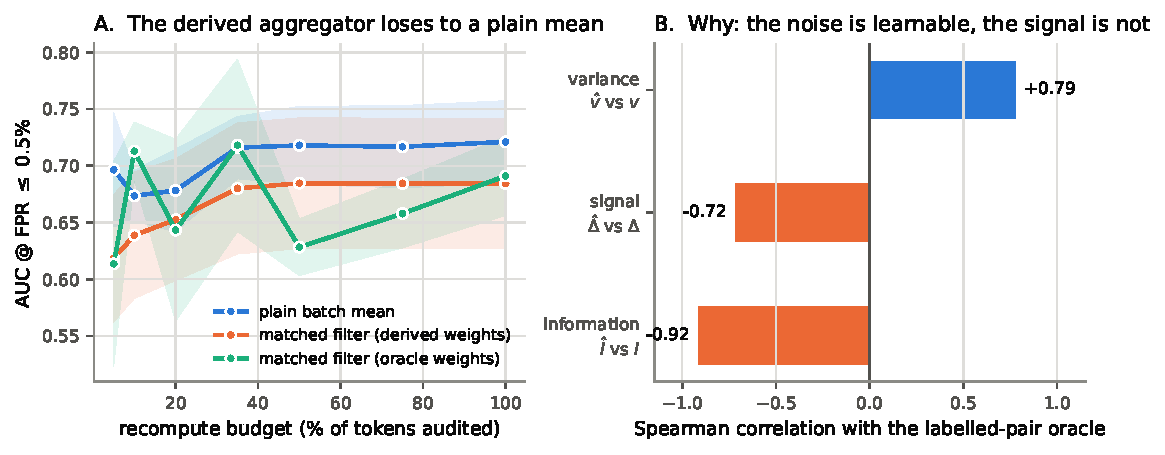
\includegraphics[width=\textwidth]{figs/fig_infodirected.pdf}
\caption{[new] Information-directed verification at full scale (Qwen3-1.7B,
\texttt{quant\_2bit}, 8{,}192-token pool, batch 400, 9 seeds). \textbf{A:} allocation
held fixed at the derived $I$ ranking so only the aggregation rule varies; the plain
mean is above the derived matched filter at every budget (bands are $\pm 1$\,sd; the
paired-by-seed test gives $t=-10.4$). \textbf{B:} the diagnosis. Rank correlation of
each estimated quantity against its labelled-pair oracle: the cheap features track the
local noise well and get the signal \emph{backwards}, so the information estimate they
imply is strongly anti-correlated with the truth.}
\label{fig:info}
\end{figure}

\textbf{Why} is the useful part, and Figure~\ref{fig:info}B is the answer. Fitting the
same nine features on labelled pairs --- labels for free, no estimation error ---
predicts the log honest variance well ($R^2 = 0.73$) and the signal not at all
($R^2 = 0.002$). Since $I = \Delta^2/v$ divides a quantity the features cannot
estimate by one they can, the resulting information estimate is not merely noisy but
\textbf{anti-correlated} with the truth (Spearman $-0.92$). The derivation is right;
the inputs it needs are not recoverable from what a client can cheaply see. Where the
deviation will show up is, on this evidence, roughly unpredictable from the proxy's
view of a position --- and a matched filter built on an anti-correlated weight estimate
is worse than no weighting at all.

\subsection{The pattern}

The prefix scheduler is a statement about prefill geometry: it holds for every value
signal, contains no statistics, and delivers $16\times$. The confidence head and the
matched filter are statements about where the evidence is, and both fail. In selective
verification, \textbf{the cost side transfers and the signal side does not} --- so the
engineering worth doing is on the accounting, not on the estimator. Anyone porting
speculative-decoding machinery into a verification setting should take the scheduler
and skip the head.

\section{What we would actually deploy}
\label{sec:deploy}

\begin{enumerate}
\item \textbf{Cascade, and put the cheap tier first for the right reason.} A
client-side proxy panel catches capability downgrades --- the attacks with real money
in them --- at a small fraction of one forward pass. Use it as a continuous
first-line filter, not as a verifier.
\item \textbf{Keep recomputation for what only recomputation can see.} Quantization,
fp8 caches, and sampler deviations are recompute-dominant; no cheap statistic reached
them in any experiment here. Spot-check with it rather than running it continuously.
\item \textbf{Use a portfolio of detectors, not the best one.} Each recompute score
is structurally blind to a different class of deviation, and which one wins is set
by the attack, not by the model --- the winning detector was identical in all six
rows of Table~\ref{tab:headline} across an 8.8$\times$ change in pool size. Run
them together. \tl{} deserves particular attention because it needs no seed
synchronization. (The cross-family sweep's claim that a portfolio lifts the floor
to 0.78 is measured at an invalid ratio; treat it as an ordering, not a level.)
\item \textbf{Budget in prefill tokens, and schedule prefixes.} A token-fraction
budget is not a cost. Depth is cheap, breadth is expensive.
\item \textbf{Spend the tuning effort on pool size, not on the estimator.} Effect
sizes here are small ($d' \approx 0.07$ for 4-bit quantization); the binding
constraint on a trustworthy verdict is how many honest tokens you have, and every
attempt to be cleverer than a plain mean failed. Size the pool before running
anything: $d'$ is cheap to measure on a few thousand tokens and tells you the batch
--- and hence the pool --- the verdict will require
(Section~\ref{sec:poolscaling}).
\item \textbf{Report the batch/pool ratio next to every AUC.} It is one number, and
without it a detection AUC is not interpretable.
\end{enumerate}

\section{Limitations}
\label{sec:limits}

\begin{itemize}
\item \textbf{Model scale.} Everything runs on a single H100, so the reference models
are 0.13B--8B. The economically interesting case is a frontier model, where the
attacker's incentive is larger, honest nondeterminism may differ, and the
proxy-to-target ratio is much smaller.
\item \textbf{Attacks are mostly simulated at the logit level.} Temperature, seed and
sampler-bug attacks are real specification changes, but quantization and fp8 caches
are applied as perturbations on top of real logits rather than by loading genuinely
quantized weights. A faithful deterministic quantization is sparse and heavy-tailed,
structurally unlike an i.i.d.\ Gaussian perturbation, even when matched on mean
divergence --- so the quantization numbers here should be read as a model of the
attack, not a measurement of it. The one genuine nf4 result we have (in the proxy
panel study) also reads chance, which is at least consistent.
\item \textbf{The verifier is passive.} No experiment here has the attacker adapting
to the specific verifier it faces, beyond the sampling-knob searches in the proxy
study. An attacker who can query the deployed detector is a strictly stronger
adversary, and the sampling-only evasions already found suggest that is where the
remaining risk is.
\item \textbf{Small-sample statistics remain the weak axis.} Five to nine protocol
seeds over pools of $10^4$ tokens can separate triage from random allocation but
cannot rank two triage signals against each other. Several comparisons in this report
are directional rather than resolved, and we have tried to label which.
\item \textbf{Most of the record is still measured over the ceiling.} We re-measured
the headline grid, the pool-scaling prediction and five cross-family cells, which is
where the load-bearing claims sit. The remaining 58 cells of the cross-family sweep,
the proxy-panel study and the confidence-head tables were not re-run at a valid
ratio, and the correction we did apply was large --- a median 0.14 AUC and up to
0.46 --- so their absolute levels should be read with the same suspicion.
Section~\ref{sec:trap} is a statement about this report as much as about the
testbed.
\item \textbf{One prompt domain, one GPU.} Cross-GPU and cross-datacenter benign
variation --- arguably the most important false-positive source in a real deployment
--- is untested, because there was only one accelerator available.
\end{itemize}

\begin{thebibliography}{9}
\small
\bibitem{difr} A.~Karvonen et al. \emph{DiFR: Inference Verification Despite
Nondeterminism}, 2025. \url{https://arxiv.org/pdf/2511.20621}
\bibitem{dspark} \emph{DSpark: Confidence-Scheduled Speculative Decoding with
Semi-Autoregressive Generation}, 2026. \url{https://arxiv.org/abs/2607.05147}
\bibitem{spec} Y.~Leviathan, M.~Kalman, Y.~Matias. \emph{Fast Inference from
Transformers via Speculative Decoding}, 2022. \url{https://arxiv.org/abs/2211.17192}
\bibitem{clymer} J.~Clymer et al. \emph{Lessons from building a model-organism
testbed}, 2025.
\end{thebibliography}

\end{document}
